\newpage
\section{Radial velocity with horizontal connection}

\subsection*{Resources}
\begin{itemize}
    \item Book sections 7/1 to 7/5
\end{itemize}

\emph{Correction to book: Figure 7/9 should read $\bm{\alpha} = \bm{\dot{\omega}} = \bm{\Omega} \bm{\times} \bm{\omega}$ (not $\bm{\Omega} \bm{\times} \bm{r}$)}

\subsection*{Challenge}
A weight ``A'' is tethered to a pole by a stiff rod of length $r$. If the angular velocity is \SI{5.5}{\radian\per\second} $\hat{k}$ and the length of the rod is \SI{47}{\meter} along the x-axis, what is the linear velocity of the weight ``A''?

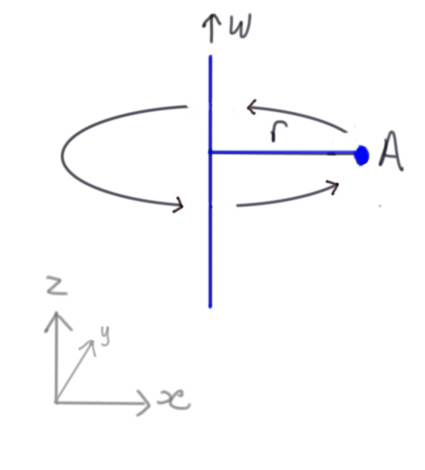
\includegraphics[height=5cm]{rod-horizontal}

\subsection*{Solution}
(Units: \si{\meter\per\second})

$\bm{\hat{i}}$\\
\soltwodp{i}{2ebd7c}\\

$\bm{\hat{j}}$\\
\soltwodp{j}{bbc682}\\

$\bm{\hat{k}}$\\
\soltwodp{k}{28435f}




\newpage
\section{Radial velocity with non-horizontal connection}

\subsection*{Resources}
\begin{itemize}
    \item Book sections 7/1 to 7/5
\end{itemize}

\emph{Correction to book: Figure 7/9 should read $\bm{\alpha} = \bm{\dot{\omega}} = \bm{\Omega} \bm{\times} \bm{\omega}$ (not $\bm{\Omega} \bm{\times} \bm{r}$)}

\subsection*{Challenge}
1. The position of ``A'' and the pole are unchanged (the radial distance is the same) and the angular velocity remains the same, but ``A'' is now hinged to the pole from below instead of horizontally, as shown in the picture. Calculate the linear velocity of ``A'' (calculate mathematically, not just by comparison with the previous challenge).

2. Write a sentence or two explaining the effect of the choice of tethering position on the calculation and the final answer.

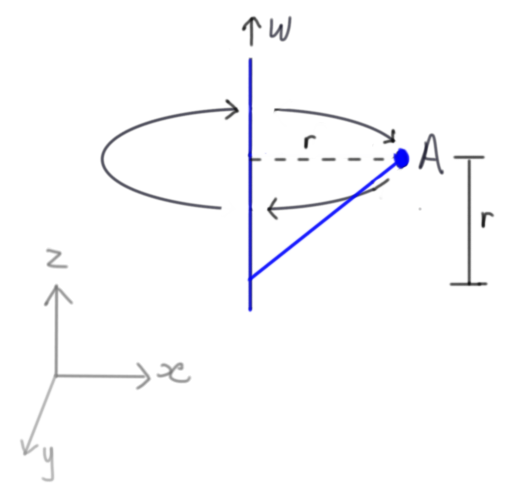
\includegraphics[height=5cm]{rod-frombelow}

\subsection*{Solution}
(Units: \si{\meter\per\second})

$\bm{\hat{i}}$\\
\soltwodp{a}{690969}\\

$\bm{\hat{j}}$\\
\soltwodp{b}{e73aa7}\\

$\bm{\hat{k}}$\\
\soltwodp{c}{11e1c5}

2. Please discuss in class if you are unsure about your answer.




\newpage
\section{Linear acceleration}

\subsection*{Resources}
\begin{itemize}
    \item Book sections 7/1 to 7/5
\end{itemize}

\emph{Correction to book: Figure 7/9 should read $\bm{\alpha} = \bm{\dot{\omega}} = \bm{\Omega} \bm{\times} \bm{\omega}$ (not $\bm{\Omega} \bm{\times} \bm{r}$)}

\subsection*{Challenge}
Using information from previous challenges, determine the:

1. Linear acceleration towards the centre of pole.

2. The tangential linear acceleration

3. Is there linear acceleration towards the centre of the pole? Is there tangential linear acceleration? Write a sentence or two to explain why for both cases.

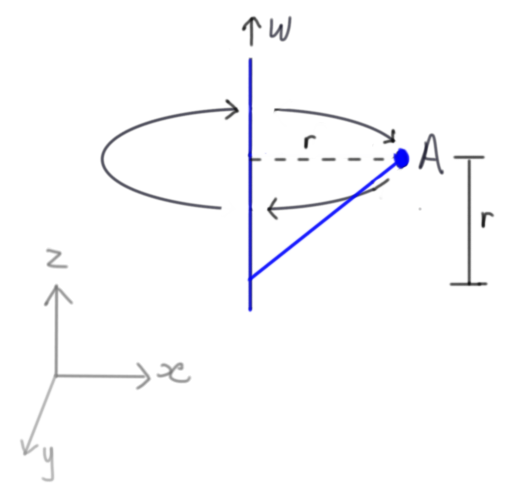
\includegraphics[height=5cm]{rod-frombelow}


\subsection*{Solution}
(Units: \si{\meter\per\square\second})

\textbf{1.}\\
$\bm{\hat{i}}$\\
\soltwodp{d}{3df1ec}\\

$\bm{\hat{j}}$\\
\soltwodp{e}{ea8d91}\\

$\bm{\hat{k}}$\\
\soltwodp{f}{645427}

\textbf{2.}\\
$\bm{\hat{i}}$\\
\soltwodp{g}{a120f7}\\

$\bm{\hat{j}}$\\
\soltwodp{h}{5a16a7}\\

$\bm{\hat{k}}$\\
\soltwodp{i}{2ebd7c}


3. Please compare your answer with your partner.




\newpage
\section{Radial acceleration - increase in magnitude of radial velocity}

\subsection*{Resources}
\begin{itemize}
    \item Book sections 7/1 to 7/5
\end{itemize}

\emph{Correction to book: Figure 7/9 should read $\bm{\alpha} = \bm{\dot{\omega}} = \bm{\Omega} \bm{\times} \bm{\omega}$ (not $\bm{\Omega} \bm{\times} \bm{r}$)}

\subsection*{Challenge}
Now consider that the radial velocity is not constant, but is undergoing an angular acceleration of \SI{2}{\radian\per\square\second}, so that the magnitude of the angular velocity $\bm{w}$ increases while it continues to point in the same direction. What is the tangential acceleration of ``A''?

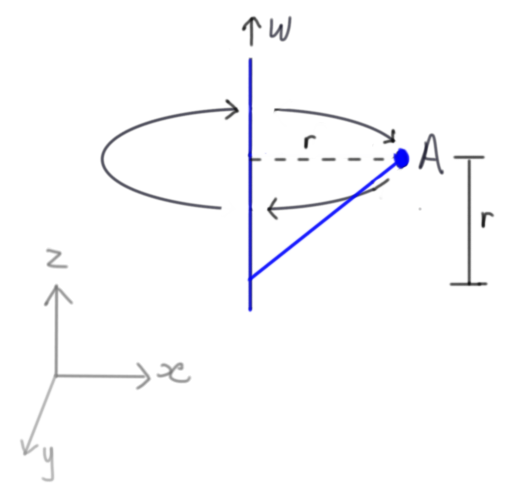
\includegraphics[height=5cm]{rod-frombelow}

\subsection*{Solution}
(Units: \si{\meter\per\square\second})

$\bm{\hat{i}}$\\
\soltwodp{m}{6d0eb9}\\

$\bm{\hat{j}}$\\
\soltwodp{n}{3c7c40}\\

$\bm{\hat{k}}$\\
\soltwodp{o}{29f8f8}




\newpage
\section{Radial acceleration - only direction (precession)}

\subsection*{Resources}
\begin{itemize}
    \item Book sections 7/1 to 7/5
\end{itemize}

\emph{Correction to book: Figure 7/9 should read $\bm{\alpha} = \bm{\dot{\omega}} = \bm{\Omega} \bm{\times} \bm{\omega}$ (not $\bm{\Omega} \bm{\times} \bm{r}$)}

\subsection*{Challenge}
The previous challenges considered the case (a) below, where the direction of the angular velocity vector $\omega$ was unchanging. Next consider that the angular velocity vector is precessing around an axis of symmetry, and this precession has an angular velocity of $\Omega$, as shown in (b). Combining (a) and (b) we have (c).

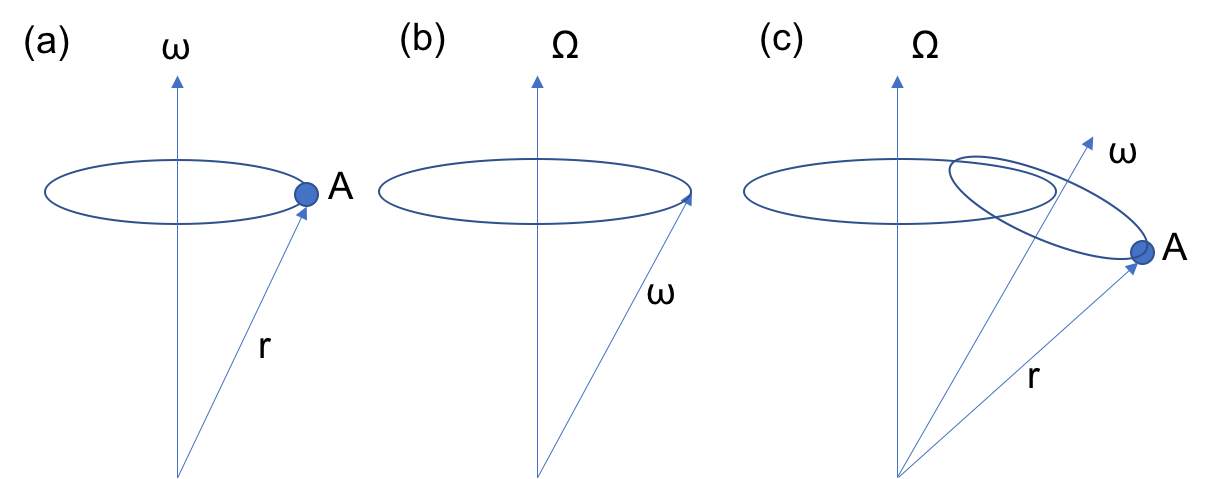
\includegraphics[height=5cm]{precession}

1. Consider the point ``A'' rotating about the vector $\omega$ with angular velocity magnitude \SI{5.5}{\radian\per\second}, but now tilt the $\omega$ vector and allow the rotation to precess around a vector of symmetry $\Omega$. Assume that only the direction (not the magnitude) of the angular velocity vector $\omega$ is changing with time. If $\Omega = 3\hat{k}$ \si{\radian\per\second} and angular velocity vector $\omega$ is inclined at \SI{45}{\degree} in the x-z plane so that the point ``A'' lays on the x-axis.

1. Calculate the linear acceleration of point ``A''.

2. Write one or two sentences to explain when the signs of the linear acceleration will be opposite but with same magnitude.


\subsection*{Solution}
1. $-3155 \hat{i} + 1005 \hat{k}$

2. Please discuss in class.




\newpage
\section{Radial acceleration II}

\subsection*{Resources}
\begin{itemize}
    \item Book sections 7/1 to 7/5
\end{itemize}

\emph{Correction to book: Figure 7/9 should read $\bm{\alpha} = \bm{\dot{\omega}} = \bm{\Omega} \bm{\times} \bm{\omega}$ (not $\bm{\Omega} \bm{\times} \bm{r}$)}

\subsection*{Challenge}
Question 7/4

\subsection*{Solution}
\SI{1285}{\meter\per\second}




\newpage
\section{Unit vector of a rotation axis}

\subsection*{Resources}
\begin{itemize}
    \item Book sections 7/1 to 7/5
\end{itemize}

\emph{Correction to book: Figure 7/9 should read $\bm{\alpha} = \bm{\dot{\omega}} = \bm{\Omega} \bm{\times} \bm{\omega}$ (not $\bm{\Omega} \bm{\times} \bm{r}$)}

\subsection*{Challenge}
Considering vector $\bm{r}$ in the figure below, if the angles $\alpha = 45$ degrees and $\beta = 30$ degrees, write the unit vector $\bm{\hat{r}}$ in terms of the Cartesian unit vectors.

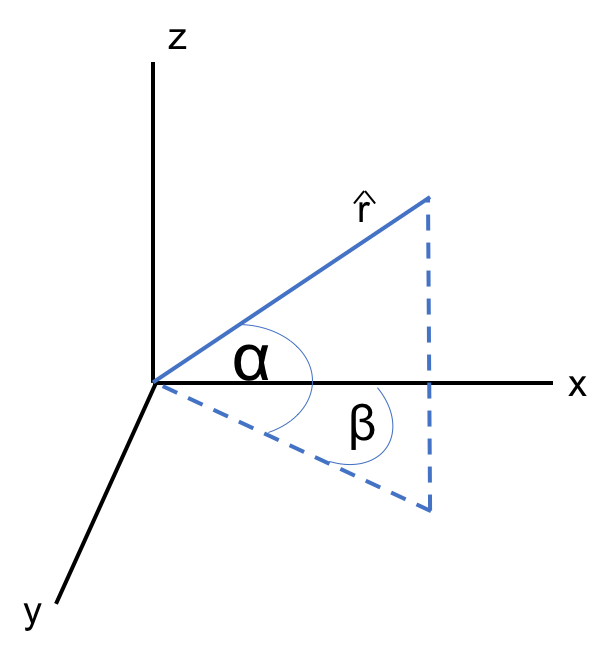
\includegraphics[height=5cm]{angles_vectors}

\subsection*{Solution}
$\bm{r} = \frac{\sqrt{3}}{2\sqrt{2}} \hat{i} + \frac{1}{2\sqrt{2}} \hat{j} + \frac{1}{\sqrt{2}} \hat{k}$


\newpage
\section{Simultaneous rotation I}

\subsection*{Resources}
\begin{itemize}
    \item Book sections 7/1 to 7/5
\end{itemize}

\emph{Correction to book: Figure 7/9 should read $\bm{\alpha} = \bm{\dot{\omega}} = \bm{\Omega} \bm{\times} \bm{\omega}$ (not $\bm{\Omega} \bm{\times} \bm{r}$)}

\subsection*{Challenge}
Work through sample problem 7/2.




\newpage
\section{Simultaneous rotation II}

\subsection*{Resources}
\begin{itemize}
    \item Book sections 7/1 to 7/5
\end{itemize}

\emph{Correction to book: Figure 7/9 should read $\bm{\alpha} = \bm{\dot{\omega}} = \bm{\Omega} \bm{\times} \bm{\omega}$ (not $\bm{\Omega} \bm{\times} \bm{r}$)}

\subsection*{Challenge}
Work through sample problem 7/1




\newpage
\section{Simultaneous rotation III}

\subsection*{Resources}
\begin{itemize}
    \item Book sections 7/1 to 7/5
\end{itemize}

\emph{Correction to book: Figure 7/9 should read $\bm{\alpha} = \bm{\dot{\omega}} = \bm{\Omega} \bm{\times} \bm{\omega}$ (not $\bm{\Omega} \bm{\times} \bm{r}$)}

\subsection*{Challenge}
Complete question 7/12


\subsection*{Solution}
Velocity: $\frac{\pi}{8}(-4 \hat{i} + 6 \hat{j} - 3 \hat{k})$ \si{\meter\per\second}

Acceleration: $\frac{\pi^2}{8}(-25 \hat{j} - 18 \hat{k})$ \si{\meter\per\square\second}




%\newpage
%\section{Time-dependent rotation of vectors I}
%
%\subsection*{Resources}
%\begin{itemize}
%    \item Book section 5/7
%\end{itemize}
%
%\subsection*{Comment}
%A vector $\bm{r}$ may be split into its magnitude and scaler components like $\bm{r} = r_i \bm{\hat{i}} + r_j \bm{\hat{j}} + r_k \bm{\hat{k}}$. For fixed co-ordinate systems, the direction of ($\bm{\hat{i}}$, $\bm{\hat{j}}$, $\bm{\hat{k}}$) does not vary with time, so the velocities of the unit vectors are zero. For a rotating co-ordinate system however, the derivative chain rule must be used in order to obtain net velocities in order to take account of the changing directions of the unit vectors.
%
%\subsection*{Challenge}
%Consider a disk spinning with angular momentum $\omega$ which itself is rotating about an axis with angular momentum $B \Omega$.
%If the angular momentum $\omega$ is increasing at a rate of A \si{\radian\per\second}, determine the net angular acceleration.
%It will be helpful to assume that the axes rotate with angular velocity $\Omega$.
%
%
%\subsection*{Solution}
%To check your answer, substitute the following values into your final equation:
%$t=1$,
%$\omega_i=10$,
%$\omega_j=3$ and
%$\omega_k=2$.
%
%Your result should be consistent with
%$\bm{\dot{\omega}} = 20 \pi \bm{\hat{i}} + 2 \bm{\hat{k}}$.




\newpage
\section{Time-dependent rotation of vectors}

\subsection*{Resources}
\begin{itemize}
    \item Book section 5/7
\end{itemize}

\subsection*{Challenge}
Answer question 7/27 in the book by:

\textbf{a)} Considering the axes fixed and not rotating with the shaft.

\textbf{b)} Considering the axes rotating with the shaft. In this case, you will need to consider the velocity components of the axes themselves as well as the velocity component induced by the swinging of the pendulum, using the derivative chain rule.

\subsection*{Solution}
The solution is given in the book and you should obtain the same answer in both cases.




%\newpage
%\section{Cross-product derivative} %NT: Move this earlier
%
%\subsection*{Challenge}
%What is the derivative of $\bm{a}(t) \bm{\times} \bm{b}(t)$ with respect to $t$?
%
%\subsection*{Solution}
%Please compare your answer with your partner and ask the teacher if you are unsure of your answer.




\newpage
\section{Relative velocity}

\subsection*{Resources}
\begin{itemize}
    \item Book section 7/6
\end{itemize}

\subsection*{Challenge}
Consider a rotating rigid body with angular velocity $\omega=\hat{k}$. Two points, ``A'' and ``B'' are chosen on the rigid body. The book describes how it is possible to calculate the velocity of point ``A'' given a set of axes (xyz) with the origin at point ``B''. Thus from the perspective of an observer on xyz, point ``A'' is rotating about point ``B''. Show that the velocity of point ``A'' relative to point ``B'' is always the same, irrespective of the choice of location of point ``B''. You may show this by demonstrating consistency for the 3 cases below.

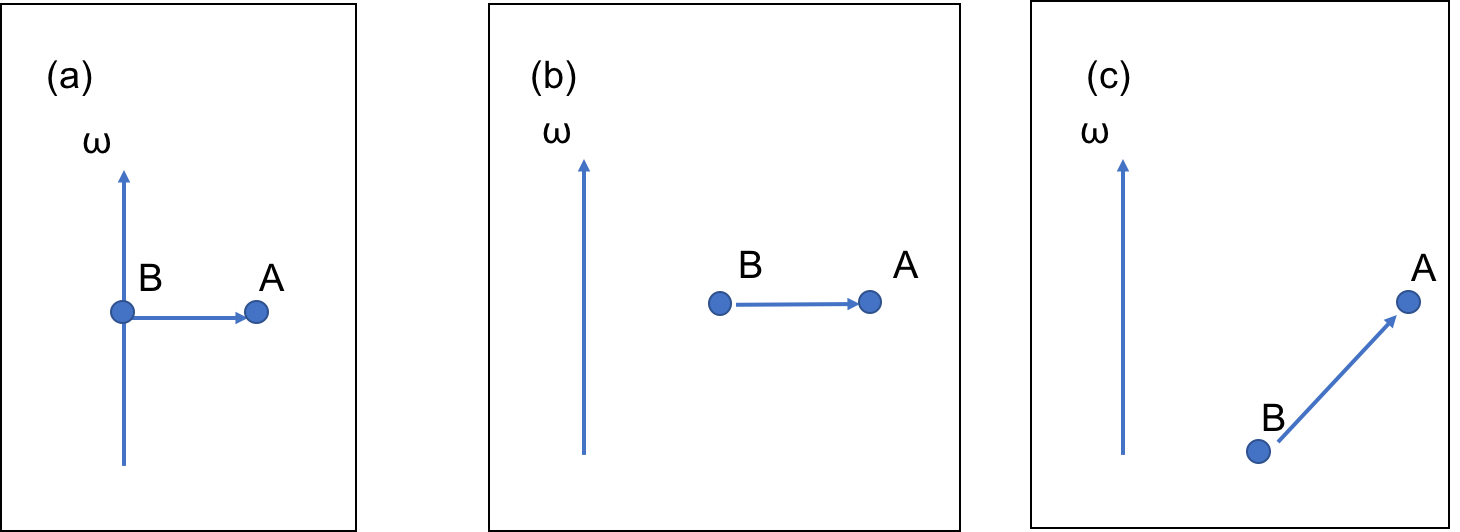
\includegraphics[width=15cm]{rigid_body_vectors}

a) $\bm{B} = \hat{k}$,              $\bm{A} = 2 \hat{i} + \hat{k}$\\
b) $\bm{B} = \hat{i} + \hat{k}$,    $\bm{A} = 2 \hat{i} + \hat{k}$\\
c) $\bm{B} = \hat{i}$,              $\bm{A} = 2 \hat{i} + \hat{k}$

\subsection*{Solution}
You should be able to show that all 3 cases will result in the same value of $v_A$. If this is not the case, please discuss with your partner or the teacher.




\newpage
\section{Crank-style problem}

\subsection*{Resources}
\begin{itemize}
    \item Book section 7/6
\end{itemize}

\subsection*{Comment}
The angular velocity of the link $\bar{AB}$ is, by definition, perpendicular to the axis of the link. In the second part of this challenge, you use this fact along with other obtained equations to obtain the 3 Cartesian directions of the angular velocity vector. Note that although the concept of the angular momentum of the link $\bar{AB}$ is used to calculate $w_2$ in the first part of the problem, you don't actually need to calculate the value of the $\bm{w_n}$ vector in order to determine the value of $w_2$.

\subsection*{Challenge}
Work through sample problem 7/3




\newpage
\section{Perpendicular position, velocity and rotation vectors}

\subsection*{Challenge}
Prove that $\bm{r}_{AB}$, $\bm{v}_{AB}$ and $\bm{\omega}_n$ in sample problem 7/3 are all perpendicular to each other. Draw a diagram to show the 3 vectors.

\subsection*{Solution}
Please compare with your partner in class.




\newpage
\section{Perpendicular double cross-product}

\subsection*{Challenge}
Considering a vector $\bm{a} = \hat{k}$ and a vector $\bm{b} = \hat{i}$, show that $\bm{a} \bm{\times} (\bm{a} \bm{\times} \bm{b}) = -a^2 \bm{b}$.




\newpage
\section{3D linear acceleration}

\subsection*{Resources}
\begin{itemize}
    \item Book section 7/6
\end{itemize}

\subsection*{Challenge}
Calculate the linear acceleration of points $A$ and $B$ in sample problem 7/4.

\section*{Solution}
$\bm{a}_A = 1800 \bm{\hat{i}} + 50 \dot{\omega_2} \bm{\hat{j}}$ \si{\mm\per\square\second}

$\bm{a}_B = 3600 \bm{\hat{k}}$ \si{\mm\per\square\second}




\newpage
\section{3D angular acceleration}

\subsection*{Resources}
\begin{itemize}
    \item Book section 7/6
\end{itemize}

\subsection*{Comment}
The last few challenges have all been building up to this challenge. This is not easy but shows how powerful the tools are that you have gained.

\subsection*{Challenge}
Work through sample problem 7/4.




\newpage
\section{3D velocity calculation}

\subsection*{Resources}
\begin{itemize}
    \item Book section 7/6
\end{itemize}

\subsection*{Challenge}
Answer question 7/38.

\subsection*{Solution}
$-0.64 \hat{i} - 4.87 \hat{j} + 1.27 \hat{k}$ \si{\meter\per\second}




\newpage
\section{3D velocity and acceleration calculation}

\subsection*{Resources}
\begin{itemize}
    \item Book section 7/6
\end{itemize}

\subsection*{Challenge}
Answer question 7/43.

\subsection*{Solution}
Given in book.




\newpage
\section{Inertia}

\subsection*{Resources}
\begin{itemize}
    \item Book appendix B
\end{itemize}

\subsection*{Challenge}
Write a paragraph describing what inertia $I$ is, explain its mathematical derivation.




\newpage
\section{Inertia: A simple cylinder}

\subsection*{Resources}
\begin{itemize}
    \item Book appendix B
    \item Video: \url{https://www.youtube.com/watch?v=Sx-5YJbszuI}
\end{itemize}

\subsection*{Challenge}
Work through sample problem B/1




\newpage
\section{Inertia: A simple sphere}

\subsection*{Resources}
\begin{itemize}
    \item Book appendix B
\end{itemize}

\subsection*{Challenge}
Work through sample problem B/2




\newpage
\section{Inertia: A 2D rectangle}

\subsection*{Resources}
\begin{itemize}
    \item Book appendix A
    \item Video: \url{https://www.youtube.com/watch?v=zhpxO0zm_E4}
\end{itemize}

\subsection*{Challenge}
Determine the area moment of inertia about the x-axis $I_x$ of a rectangle which is centred on the x-y axes with x and y lengths ``X'' and ``Y'' respectively.

\subsection*{Solution}
You should find that your answer is consistent with $I_x = 2$ for $X=3$ and $Y=2$.
%\begin{equation}
%    \frac{XY^3}{12}
%\end{equation}




\newpage
\section{Inertia: A simple parallelepiped}

\subsection*{Resources}
\begin{itemize}
    \item Book appendix B
\end{itemize}

\subsection*{Challenge}
Work through sample problem B/3




\newpage
\section{Inertia: A cone}

\subsection*{Resources}
\begin{itemize}
    \item Book appendix B
\end{itemize}

\subsection*{Challenge}
Answer question B/4

\subsection*{Solution}
Your solution should be consistent with a total mass of \SI{8}{\kg} and a radius of \SI{3.5}{\meter} having an intertia $I_{zz}$ of \SI{49}{\kg\meter^2}.




\newpage
\section{Inertia: A rod}

\subsection*{Resources}
\begin{itemize}
    \item Book appendix B
\end{itemize}

\subsection*{Challenge}
Answer question B/3

\subsection*{Solution}
Given in book.




\newpage
\section{Inertia: A rod and a disk}

\subsection*{Resources}
\begin{itemize}
    \item Book appendix B
\end{itemize}

\subsection*{Challenge}
Answer question B/18. Please fully derive your answer, except you may use the fact that $I_{xx}$ for each rod is $m L^2/6$.

\subsection*{Solution}
Your answer should be consistent with a length of \SI{1.73}{\meter} for a disk radius of \SI{2}{\meter}.




\newpage
\section{Inertia: A bent cylinder}

\subsection*{Resources}
\begin{itemize}
    \item Book appendix B
    \item Book appendix D
\end{itemize}

\subsection*{Challenge}
Answer question B/27. You do not need to derive solutions from first principles, and instead may refer to appendix D to build your answer.

\subsection*{Solution}
Given in book.



\iffalse
\newpage
\section{Off-diagonal inertia}

\subsection*{Resources}
\begin{itemize}
    \item \url{https://www.colorado.edu/physics/phys3210/phys3210_fa15/lecnotes.2015-10-14.The_Inertia_Tensor.html}
\end{itemize}

\subsection*{Challenge}
Consider a cube. The x, y an z axes pass through the centre of the cube perpendicular to the faces of the cube (ie, each axis passes through the centre of a face). The mass of the cube is evenly distributed so the centre-of-mass of the cube is in the centre, where the 3 axes cross.

The off-diagonal values of inertia $I_{xy}$, $I_{xz}$ and $I_{yz}$ are zero. Show this mathematically.

\subsection*{Solution}
Please compare your answer with your partner.




\newpage
\section{Angular momentum and kinetic energy of two plates}

\subsection*{Resources}
\begin{itemize}
    \item Book section 7/7 and 7/8
\end{itemize}

\subsection*{Challenge}
Work through sample problem 7/6.




\newpage
\section{Angular momentum and kinetic energy of a cone}

\subsection*{Resources}
\begin{itemize}
    \item Book section 7/7 and 7/8
\end{itemize}

\subsection*{Challenge}
Answer question 7/65. Note that the question only concerns the cone, and not the cone-rod system.

\subsection*{Solution}
Given in book.




\newpage
\section{Angular momentum and kinetic energy of a rolling disk}

\subsection*{Resources}
\begin{itemize}
    \item Book section 7/7 and 7/8
\end{itemize}

\subsection*{Challenge}
Answer question 7/71.

\subsection*{Solution}
Given in book.
\fi
